%! Author = Runge
%! Date = 29-12-2023

% Preamble
\documentclass[english,a4paper,compsoc,journal]{IEEEtran}
\overfullrule=10pt
\frenchspacing

% Packages
%! Author = Runge
%! Date = 29-12-2023

% Packages
\RequirePackage{setup/clrscode4e}
\usepackage{amsmath}
\usepackage{amsthm}
\usepackage{amssymb}
\usepackage{amsbsy}
\usepackage{mathrsfs}
\usepackage{dsfont}
\usepackage{bbold}
\usepackage{booktabs}
\usepackage{tikz}

% Packages with options set
\usepackage[hidelinks]{hyperref}
\usepackage[textsize=small,obeyDraft]{todonotes}
\usepackage[newfloat]{minted}
\usepackage[backend=biber,
    bibencoding=utf8,
    maxbibnames=20,
    style=ieee,
    citestyle=numeric-comp,
    url=false
]{biblatex}
\usepackage[acronym]{glossaries}

% Package setup
\setlength{\marginparwidth}{2cm} % todonotes width
\setminted{linenos, autogobble, breaklines, fontsize=\footnotesize, style=friendly, xleftmargin=1em, numbersep=5pt}
\addbibresource{bib/main.bib}

% Other setup and options
\newtheorem{theorem}{Theorem}
\newtheorem{definition}{Definition}
\newfloat{algorithm}{htb!}{lop}
\floatname{algorithm}{Algorithm}
\newcommand{\algorithmautorefname}{Algorithm}

\makeglossaries

%! Author = Runge
%! Date = 29-12-2023

\newacronym{aau}{AAU}{Aalborg University}
\newacronym{zkp}{ZKP}{Zero-Knowledge Proof}
\newacronym{pos}{PoS}{Proof of Stake}
\newacronym{pow}{PoW}{Proof of Work}
\newacronym{zk-snark}{ZK-SNARK}{Zero-Knowledge Succinct Non-Interactive Argument of Knowledge}
\newacronym{zk-stark}{ZK-STARK}{Zero-Knowledge Scalable Transparent Argument of Knowledge}
\newacronym{zk-rollup}{ZK-rollup}{Zero-Knowledge Rollup}
\newacronym{maci}{MACI}{Minimum Anti-Collusion Infrastructure}
\newacronym{ssle}{SSLE}{Single Secret Leader Election}
\newacronym{lmd}{LMD}{Latest Message Driven}
\newacronym{ghost}{GHOST}{Greedy Heaviest Observed Subtree}
\newacronym{poc}{PoC}{Proof-of-Concept}
\newacronym{lmd-ghost}{LMD-GHOST}{Latest Message Driven Greedy Heaviest Observed Subtree}
\newacronym{randao}{RANDAO}{random number generator}
\newacronym{dos}{DoS}{Denial-of-Service}
\newacronym{enr}{ENR}{Ethernet Node Record}
\newacronym{p2p}{P2P}{Peer-to-Peer}
\newacronym{de-anon paper}{De-anonymizing Paper}{"Deanonymizing Ethereum Validators: The P2P Network Has a Privacy Issue"}
\newacronym{mev}{MEV}{Maximal Extractable Value}
\newacronym{ddh}{DDH}{Decisional Diffie-Hellman}
\newacronym{ipa}{IPA}{Inner Product Argument}
%! Author = Runge
%! Date = 29-12-2023

\title{Zero-Knowledge Proof for attack prevention in the Ethereum Blockchain}

\author{\IEEEauthorblockN{Anders Malta Jakobsen}
\IEEEauthorblockA{\textit{dept. of Computer Science} \\
\textit{AAU}\\
Aalborg, Denmark \\
amja23@student.aau.dk}\\
\and
\IEEEauthorblockN{Oliver Holmgaard}
\IEEEauthorblockA{\textit{dept. of Computer Science} \\
\textit{AAU}\\
Aalborg, Denmark \\
oholmg20@student.aau.dk}
}


% Document
\begin{document}
    \onecolumn     % switch to one‐column formatting
\thispagestyle{empty}

\begin{center}
    \begin{tcolorbox}[
        width=\dimexpr\paperwidth - 2in\relax,  % span from 1" margin to 1" margin
        colback=white,                          % white background
        colframe=white,                         % black border
        left=60pt, right=60pt, top=10pt, bottom=10pt, % internal padding
        boxrule=0.8pt, % thickness of border line
        fontupper=\large
    ]
        \textbf{\large Summary}%

This paper addresses a key vulnerability in Ethereum’s proof-of-stake (PoS) protocol, namely the vulnerability of block proposers against denial-of-service (DoS) attacks.
This is made possible through deanonymization, where adversaries get validator IP addresses, after which they check for matches and attack upcoming proposers.
To counter this, Ethereum has proposed the Whisk protocol, a Single Secret Leader Election (SSLE) protocol that uses zero-knowledge proofs to hide proposer identities.
Whisk is shuffle-based, meaning it resists adversarial tracking by iteratively shuffling a subset of a list of trackers, where each validator has a single tracker.
Each shuffle in Whisk relies on a shuffle-based zero-knowledge proof called Curdleproofs, which uses Inner Product Arguments (IPAs) to validate the correctness of the shuffle.
However, Curdleproofs is constrained to shuffling subsets of sizes that are only a power of two due to the recursive nature of the IPA.


This is why we propose a modified protocol, CAAUrdleproofs, which lifts this restriction by integrating ideas from Springproofs.
CAAUrdleproofs introduces a new folding scheme which allows the use of arbitrary shuffle sizes to enable more flexibility when reducing or increasing the size.
The experiments show that CAAUrdleproofs maintains similar performance to Curdleproofs for power of two shuffle sizes but outperforms it when shuffle sizes are not a power of two; especially when the size is slightly above a power of two.
This paper also proposes reducing the shuffle size from 128 down to 80 which would result in a notable decrease in the block overhead created by the protocol.
The overhead would go from 16.656 KB to 12.048 KB, saving around 12.11 GB annually.


This paper also provides security analysis of the shuffle mechanism with different shuffle sizes and under various amounts of adversarial influence.
The results validate that smaller shuffle sizes can still maintain a secure shuffle within the Amount available to the protocol.
The paper concludes by mentioning that CAAUrdleproofs is an efficient improvement to Curdleproofs, and it suggests future development in the directions of post-quantum security, protocol refinement or possibly looking at the use of Weighted inner product argument (WIPA).



        \end{tcolorbox}
    \end{center}
    \clearpage
    \setcounter{page}{1}
    \twocolumn
    \maketitle
    
\begin{abstract}
    Ethereum is one of the leading Proof-of-Stake blockchains.
    However, it is still vulnerable to attacks.
    One such attack is the de-anonymization attack by Heimbach et al.~where an adversary could get validator IP addresses and then perform a denial-of-service attack on them.
    To try and combat this attack, Ethereum has proposed the use of the Whisk protocol.
    Whisk is a Single Secret Leader Election protocol that uses a zero-knowledge proof called Curdleproofs that uses Inner Product Arguments to prove the validity of a shuffle of validators.
    This paper improves upon Curdleproofs' Inner Product Arguments by introducing CAAUrdleproofs, which is a modified version of Curdleproofs with ideas from Springproofs as to overcome the limitations of Curdleproofs regarding the shuffle size.
    We show that CAAUrdleproofs has similar proving and verifying times to Curdleproofs when the shuffle size is a power of two.
    We also show that CAAUrdleproofs has a performance advantage for any shuffle size that is not a power of two, and that this advantage grows the lower the shuffle size is below a power of two.
    After performing experiments, we also suggest a new shuffle size which is smaller than the current one used in Curdleproofs that would result in a smaller block overhead than the one created by the current Curdleproofs protocol.
    All this is done while still preserving the anonymity of validators.

\end{abstract}

\begin{IEEEkeywords}
    Ethereum, Proof of Shuffle, Distributed Systems, Inner Product Arguments, Zero-Knowledge Proof, Single Secret Leader Election
\end{IEEEkeywords}

    

\section{Introduction}\label{sec:introduction}
Ethereum is a decentralized blockchain platform that enables developers to build and deploy smart contracts and decentralized applications.
It is the second-largest blockchain platform by market capitalization and has a large and active developer community.
Currently working as a Proof-of-Stake protocol, it allocates block proposal opportunities to the ones in the community willing to stake their ether; also called validators.
Though, previous work from Heimbach et al., confirmed by ourselves, shows that adversaries are able to gather validator IP addresses~\cite{heimbach2024deanonymizingethereumvalidatorsp2p,ouroldpaper}.
These can be used to perform a Denial-of-Service (DoS) attack on the validators, threatening the liveness of the blockchain~\cite{EthereumAttackDefense2024,ouroldpaper}.

In response to the potential threat, Ethereum has proposed a protocol, Whisk, which hides validators' identities making the DoS attack harder to perform~\cite{Whisk2024}.
Whisk is a Single Secret Leader Election protocol~\cite{10.1145/3419614.3423258}, where validators each publish a private tracker, which is used for proposer selection instead.
When proposing a block, the validator will then prove the ownership of the tracker.
To ensure that adversaries are unable to trace the tracker to specific validators, each block proposer shuffles the list of validator trackers while adding randomness to the trackers.

Making sure that this has been done correctly is essential to the protocol.
Hence, Whisk uses a proof protocol, called Curdleproofs, which is a Zero-Knowledge proof of shuffle~\cite{Curdleproofs}.
Therefore, the block proposer constructs such a proof, adds it to the block, after which other validators can verify the proof.

This introduces block size overhead to the blockchain.
Also, additional work is required for both provers and verifiers.

In this paper, we dive into the structure of Curdleproofs to understand, where the protocol can be optimized.
Specifically, we work with the concept of Inner Product Arguments and how they generally only work for vector sizes that are powers of two.

Our protocol, CAAUrdleproofs, aims to improve on the rigid nature of Curdleproofs.
Following this, we also provide argumentation of when CAAUrdleproofs is still secure.

Working with this led to the following contributions:
\begin{itemize}
    \item We have successfully modified Curdleproofs, using the Springproofs framework~\cite{zhang2024springproofs}, to allow flexibility when choosing the shuffle size.
    \item We have implemented CAAUrdleproofs and run experiments on both protocols, showing that CAAUrdleproofs has potential to be faster and smaller in size compared to Curdleproofs.
    \item We have experimentally provided argumentation that CAAUrdleproofs is still secure when lowering the size of shuffled elements.
\end{itemize}



    
\section{Background}\label{sec:background}
In this section, we will go through some of the concepts that will be used in the rest of the paper as well as some surrounding context for the attack.

\subsection{Ethereum and Proof of Stake}\label{subsec:ethereum-and-proof-of-stake}
Ethereum is a blockchain platform that allows developers to create decentralized applications using smart contracts.
Previously operating with a~\gls{pow} consensus algorithm, Ethereum transitioned to a~\gls{pos} consensus algorithm in 2022.
This transition was done to reduce the energy consumption of the network and to increase the scalability of the network.
The transition was done in a series of upgrades called the Ethereum 2.0 upgrade.
~\gls{pos} is a consensus algorithm that is used to secure blockchain net by helping to create new blocks and confirm transactions.
It works by creating validators based on the amount of cryptocurrency they have staked.
Then it selects some of these validators as proposers to be the ones to create new blocks, which then are confirmed by the rest of the validators.
The proposers then get rewarded for creating a valid block and the validators get rewarded for confirming the block.
Block proposing happens within epochs of 32 blocks per epochs and for each epoch a group of validators is selected and from them a proposer is chosen.
the way the proposer is chosen is through a random proses that is weighted by the amount of cryptocurrency the validator has staked, and by using the publicly available \gls{randao} algorithm to simulate the random selection.
The blocks also have a time limit of 12 seconds to be created and confirmed else the block will be discarded and the proposer is penalized.
If a fork happens the validators have to choose which fork to follow.
This is done by using the \gls{lmd-ghost} algorithm which chooses the fork with the greatest weight of attestations in its history~\cite{EthereumProof-of-stakePoS}.

\subsection{subnets}\label{subsec:subnets}
The Ethereum network is split up into smaller networks called subnets.
Being subscribed to a subnet is also be referred to as being backbone of a subnet.
These subnets are used to help with the scalability of the network.
The nodes in the network are split into total of 64 subnets and an additional subnet for attestation aggregates with each node being part of at least two subnets.
Within a subnet, nodes choose a subset of peers in the same subnet to share its messages with.
Choosing which notes are a part of this subset is done based on the peers performances.
Nodes send all messages they hear about within a subnet to these best-performing peers.
The peers a node can reach within the same subnet is called its fanout~\cite{heimbach2024deanonymizingethereumvalidatorsp2p}.



%\subsection{Zero-Knowledge Proofs}\label{subsec:zero-knowledge-proofs}
%A~\gls{zkp} is a cryptographic method that allows one party to prove to another party that something is true without revealing any information.
%
%Two of the subcategories of \gls{zkp}s are \gls{zk-snark} and \gls{zk-stark}.
%~\gls{zk-snark} is the more common of the two.
%It uses elliptic curve cryptography to create proofs based on the assumption that it is hard to find the discrete logarithm form the publicly known base point.
%~\gls{zk-snark} has a start-up ritual which requires a trusted setup by all parties involved that the original proving key is destroyed as to not be able to create fake proofs.
%A criticism of \gls{zk-snark} is that it is not quantum resistant because of the reliance on elliptic curve cryptography.
%
%~\gls{zk-stark} on the other hand, is a newer and more complex~\gls{zkp}.
%Despite not having non-interactive in its name,~\gls{zk-stark} is also non-interactive.
%Different form~\gls{zk-snark},~\gls{zk-stark} uses hashing functions to create proofs instead of elliptic curves.
%This method is post-quantum secure and does not require a trusted setup.
%It does, however, come with a higher computational cost and is not as widely used and documented as~\gls{zk-snark}.

\subsection{Validators}\label{subsec:validator}
Our attack is primarily focused on the validators of Ethereum.
A validator is an entity running on a validator client,
which, among other things, consists of a balance and a key-pair for identifying it~\cite{Staking}.
One client can run several validators.

The validators have a central job in keeping the blockchain running.
At each slot, a validator in Ethereum is at random chosen to be responsible for processing transactions,
including them in a block,
and then adding this block to the blockchain.
How we determine who is going to be a block proposer will be explained in~\autoref{subsec:randao}.
Along with this, the validator is also responsible for attesting blocks proposed by other validators,
ensuring the liveness of the chain.

To be able to have a single validator, one must deposit 32 ETH,
which is ~\$99,776\footnote{As of 2024-11-18 seen on \href{https://beaconcha.in/}{beaconcha.in}}.
Having this much money at stake should be enough to ensure that a validator acts honestly.
Doing so will also earn the validator a reward, but contrary to that,
acting dishonest will get you ETH burned or slashed.
The rewards and punishments will be described in the following.
\subsubsection{Validator rewards}\label{subsubsec:valrewards}
Validators are rewarded for several different actions~\cite{PoSRewAndPen}.
Each of these actions is rewarded with different weights,
but they all depend on the total amount of staked ETH by validators and the validator's own staked amount limited to 32 ETH\@.
A base reward, which is used on the reward weights, is calculated for a single validator as follows:
\begin{equation}
    BR = EB\cdot(\frac{BRF}{BRPE\cdot \sqrt{\sum{AB}}})
    \label{eq:basereward}
\end{equation}, where \texttt{BR} is \textit{base reward},
\texttt{EB} is \textit{effective balance}, \texttt{BRF} is \textit{base reward factor} set to 64,
\texttt{BRPE} is \textit{base rewards per epoch} set to 4,
and \texttt{AB} is \textit{active balance}, which is the total staked ETH by validators.

The reward for a validator is then calculated as follows:
\begin{equation}
    \frac{\sum{weights}}{64}\cdot BR
    \label{eq:valrewards}
\end{equation}
The summed over weights are the following:
\begin{enumerate}
    \item Timely source vote: 14
    \item Timely target vote: 26
    \item Timely head vote: 14
    \item Sync reward: 2
    \item Proposer weight: 8
\end{enumerate}
Though not the highest weight, the most profitable reward is actually the proposer weight reward.
The validator is rewarded with this, whenever they are chosen and correctly propose a block to the blockchain.
But instead of being rewarded this only once,
the proposer is getting the reward as many times as there are attestations.
\begin{equation}
    BR\cdot\frac{8}{64}\cdot \#attestations\label
    {eq:propreward}
\end{equation}
Because the maximum number of attestations is 128,
then in a typical and optimal situation,
the proposer will get $BR\cdot\frac{8}{64}\cdot128$ in reward
when proposing a block~\cite{PoSRewAndPen,consensus-spec-phase-0}.
Thus, with the average amount of staked ETH for a validator being over 32 ETH, which means almost equal chance of being proposer, and with Ethereum having over 1 million validators, validators do not want to miss being the proposer\footnote{As of 2024-11-18 seen on \href{https://beaconcha.in/}{beaconcha.in}}.

\subsubsection{Validator punishments}\label{subsubsec:valpunish}
A validator can also be punished for doing things that do not contribute to the chain performing as it should.
Ethereum has two kinds of penalties, burning and slashing, where a validator loses some of their staked ETH\@.
Should a validator lose their ETH and end up below 16 staked ETH, they will be removed~\cite{consensus-spec-phase-0}.


Burning happens per epoch when a validator is offline.
If ETH gets burned, it is gone forever.
To calculate how much ETH is retained after burning per offline epoch, ~$n$, the following formula is used:
\begin{equation}
    \left(1-\frac{1}{IPQ}\right)^\frac{n^2}{2}
    \label{eq:burn}
\end{equation},
with \texttt{IPQ} being the \textit{inactivity penalty quotient} set to $2^{26}$~\cite{consensus-spec-phase-0}.


This means that a validator being offline in a single epoch still retains $0,99999999255\%$ of their staked ETH\@.
A validator would therefore need
to be offline for a lot of epochs before eventually being removed for having under 16 staked ETH\@.


Slashing happens when only when a validator acts maliciously against the blockchain,
and cannot be invoked only by being offline.
Slashing happens from at least one of three causes~\cite{PoSRewAndPen}:
\begin{enumerate}
    \item Proposing two different blocks at the same slot
    \item Attesting a block that surrounds another
    \item Double voting - Attesting to candidates for the same block
\end{enumerate}
If this is detected, ~$\frac{1}{32}$ of the validator's staked ETH is immediately burned,
and a 36-day removal period of the validator begins, where the staked ETH is gradually burned.
Halfway through this, on day 18, an additional penalty is applied.
The magnitude of this penalty scales with the total staked ETH of the slashed validators in the 36-day period before the slashing event.
At worst, a validator can end up having all their ETH burned, if enough other validators are also slashed.

\subsection{RANDAO}\label{subsec:randao}

\subsection{ENR}\label{subsec:enr}
A~\gls{enr} is a record that contains information about a node in the network~\cite{EIP-778:Ethereum-Node-Records}.
Ethereum uses~\glspl{enr} as a way
to package the information that is being sent from node to node during the discovery protocol,
where nodes discover each other.
The package contains information like the node's IP address, port, and public key.
Because of the nature of the discovery protocol, if you where to also be a node in Ethereum,
you would be able to see the~\gls{enr} of all the nodes that you have discovered.
And since the~\gls{enr} contains the IP address and the public key of the node,
you would be able
to see the corresponding IP addresses and public keys of all the nodes that have been discovered by the node.


\subsection{other paper}\label{subsec:other-papers} \todo{new titel}
\todo{make acronym for the paper}
In the paper "Deanonymizing Ethereum Validators: The P2P Network Has a Privacy Issue" the authors show that it is possible to deanonymize validators on the Ethereum network by observing attestations and subscribing to subnets~\cite{heimbach2024deanonymizingethereumvalidatorsp2p}.
This paper is relevant to our work as it shows that it is possible to get information about the validators on the network.
This paper is also the main inspiration for our attack.
The paper takes advantage of the attestations, including information such as the IP of the sender node, and subnet setup to get information about the validators.
For their setup they use a custom version of a Prysm node called RAINBOW that subscribe to all subnets, and they use to log and color the information gathered.
This information consists of all attestations, their origin, and their origin subnet, all advertised static subscriptions of our peers and precise connection data for all nodes we interact with.
To help speed up the discovery of the peers they also used a crawler to more quickly find the peers using the discovery protocol and the peer tables.
In their execution of their experiment they set up four nodes spread out across four different geographical locations.
They then let the nodes run for three days and managed to deanonymize 235,719 validators and reached out to 11,219 peers.
These peers were also divided into 4 categories based on their heuristic.
Those being deanonymized where they located validators on the machine with the heuristic conditions being upheld, No validators where they did not receive a single non-backbone attestation received from the peer, and so they assume that there are no validators on the peer, 64 subnets where they never receive a non-backbone attestation from the peer which makes it impossible to deanonymize the validators and the rest where they got at least one non-backbone attestation but where not able to locate any validators on the peer.




\subsection{Proposer DoS Attack}\label{subsec:proposer-dos-attack}
In this subsection, we will be describing the attack that we will be using as a basis for our experiment in ~\autoref{sec:experimental-protocol}.
The attack is a~\gls{dos} attack that aims at hitting the proposers selected for creating blocks in the chain.
Ethereum themselves have mentioned it as a potential attack, and with the current implementation of the consensus algorithm, it seems that this attack is possible to perform~\cite{EthereumSSLE2024,EthereumAttackDefense2024}.

It has been our interest to research the feasibility of this attack and the ones mentioned in~\autoref{sec:attacks-on-ethereum}.
This has proven to be a difficult task, given that most of our researched attacks happen in the consensus- or execution layer.
Therefore, as a result of the blockchain algorithm, we are not able to clarify the feasibility of the attacks that we have found.
For this reason, we have chosen the \textit{Proposer~\gls{dos} attack} as it seems exciting, has not been mitigated yet, and a potential solutions seems to include a~\gls{zkp}.
%\todo{Does it make sense to mention \# skipped blocks pr day even though we are unsure if any of these are attacks}

The attack possible is because the consensus mechanism uses a publicly known function for choosing the upcoming block proposers.
The adversary is therefore able to compute this in slight advance of the blockchain, s.t.\ each proposer is now known.
After this, the adversary can map the proposer's IP addresses and overload their connection.
A successful attack would leave a proposer unable to propose their block in time.\todo{Should possibly be explained in more detail}
    

\section{Related Work}\label{sec:related-work}
The usage of~\glspl{zkp} in Ethereum is not a new concept.
In fact, it currently uses them both on- and off-chain.
The following provides a short overview of some of the already existing solutions as well as one still being in development.

%\subsection{Off-chain roll-ups}\label{subsec:off-chain-roll-ups}
%As a result of Ethereum's popularity, the network could easily get congested if developers were not actively trying to distribute computations~\cite{EthereumScaling2024}.

%One of the first ideas was to introduce an on-chain technique called sharding.
%It is a technique where the database would be split into different parts between subsets of validators.
%Sharding was never deployed on the blockchain though, and instead Ethereum uses off-chain solutions to off-load computations.
%The idea of off-chain solutions, called L2-roll-ups, is that users commit their work to off-chain nodes.
%These perform the computations, thereafter they submit the work to the Ethereum Mainnet chain.
%
%One of these solutions is called a~\gls{zk-rollup}.

\subsection{dos attack}\label{subsec:dos-attack}
Some of the instances of dos attacks that is seen on ethereum ranges from attacks on the proposers to attacks that seek to slow down the network itself.
A known attack aims to slow down the network by using underpriced opcodes to create a block that is hard to process~\cite{10.1145/3391195,9815256}.
Another way to slow down the network is to create empty accounts that are hard to process~\cite{empty-account-mitigation,empty-account-eip-mitigation}.
This attack however is outdated and has been mitigated by making at near impossible to create empty accounts in the network.


    \input{sections/04-approach}
    
\section{Experimental Protocol}\label{sec:experimental-protocol}
In this section, we will describe how our experiments are run, and what we want to measure.
We also discuss which parameters we can tweak in the different experiments that we have.

The experiments are run on a virtual machine hosted on Strato CLAAUDIA through Aalborg University.
The machine is using an Intel Xeon Cascadelake processor, CPU family 6, model 85.
It has 16 virtual CPUs and 64 GB of RAM available.
The virtual machine is running Ubuntu Server 24.


\subsection{CAAUrdleproof}\label{sec:CAAUrdleproof-experiment}
In this experiment we measure the time to run the CAAUrdleproofs protocol.
The results will be compared to those of Curdleproofs, which we re-run on our own hardware.
As Curdleproofs already has a Rust benchmark implemented, we will be using that same benchmark for both protocols.
The parameter that we want to change between benchmark runs is the shuffle size, $\ell$.

In CAAUrdleproofs, we will test the protocol with $\ell=\{8,9,\dots,256\}$.

Since Curdleproofs is unable to run benchmarks, unless the shuffle size is a power of two, those benchmarks will be run on values $\ell=\{8,16,32,64,128,256\}$.




\subsection{Shuffle security}\label{subsec:experimental-protocol-shuffle-security}
In this experiment we run the shuffle protocol with varying shuffle sizes and varying number of adversarial tracked ciphertexts.
The purpose of this experiment is to find the lowest possible shuffle size that is still secure.
We therefore run the experiment with shuffle sizes, $\ell$, between 64 and 128.
For the number of adversarial tracked ciphertexts, we use the values $\alpha=\{1/2,1/3,1/4\}$

Because Curdleproofs is meant to be used in an Ethereum setting, all the experiments were done with a maximum of 8192 shuffles.
Also, the experiments shuffle over a set of 16,384 ciphertexts.
Both of these numbers come from the Ethereum Whisk proposal~\cite{Whisk2024}.


Every experiment is run 1000 times to avoid statistical uncertainty.
As done by the shuffle authors~\cite{cryptoeprint:2022/560}, we will denote the 20th, 40th, 60th, 80th, and 100th percentile on when the shuffle is deemed secure by the experimental runs.


    \section{Results}\label{sec:results}




\subsection{Proving and Verifying Times}\label{subsec:results:provingverifying}
\begin{figure*}[!ht]
    \centering
    \subfloat[\centering Proving Time]{{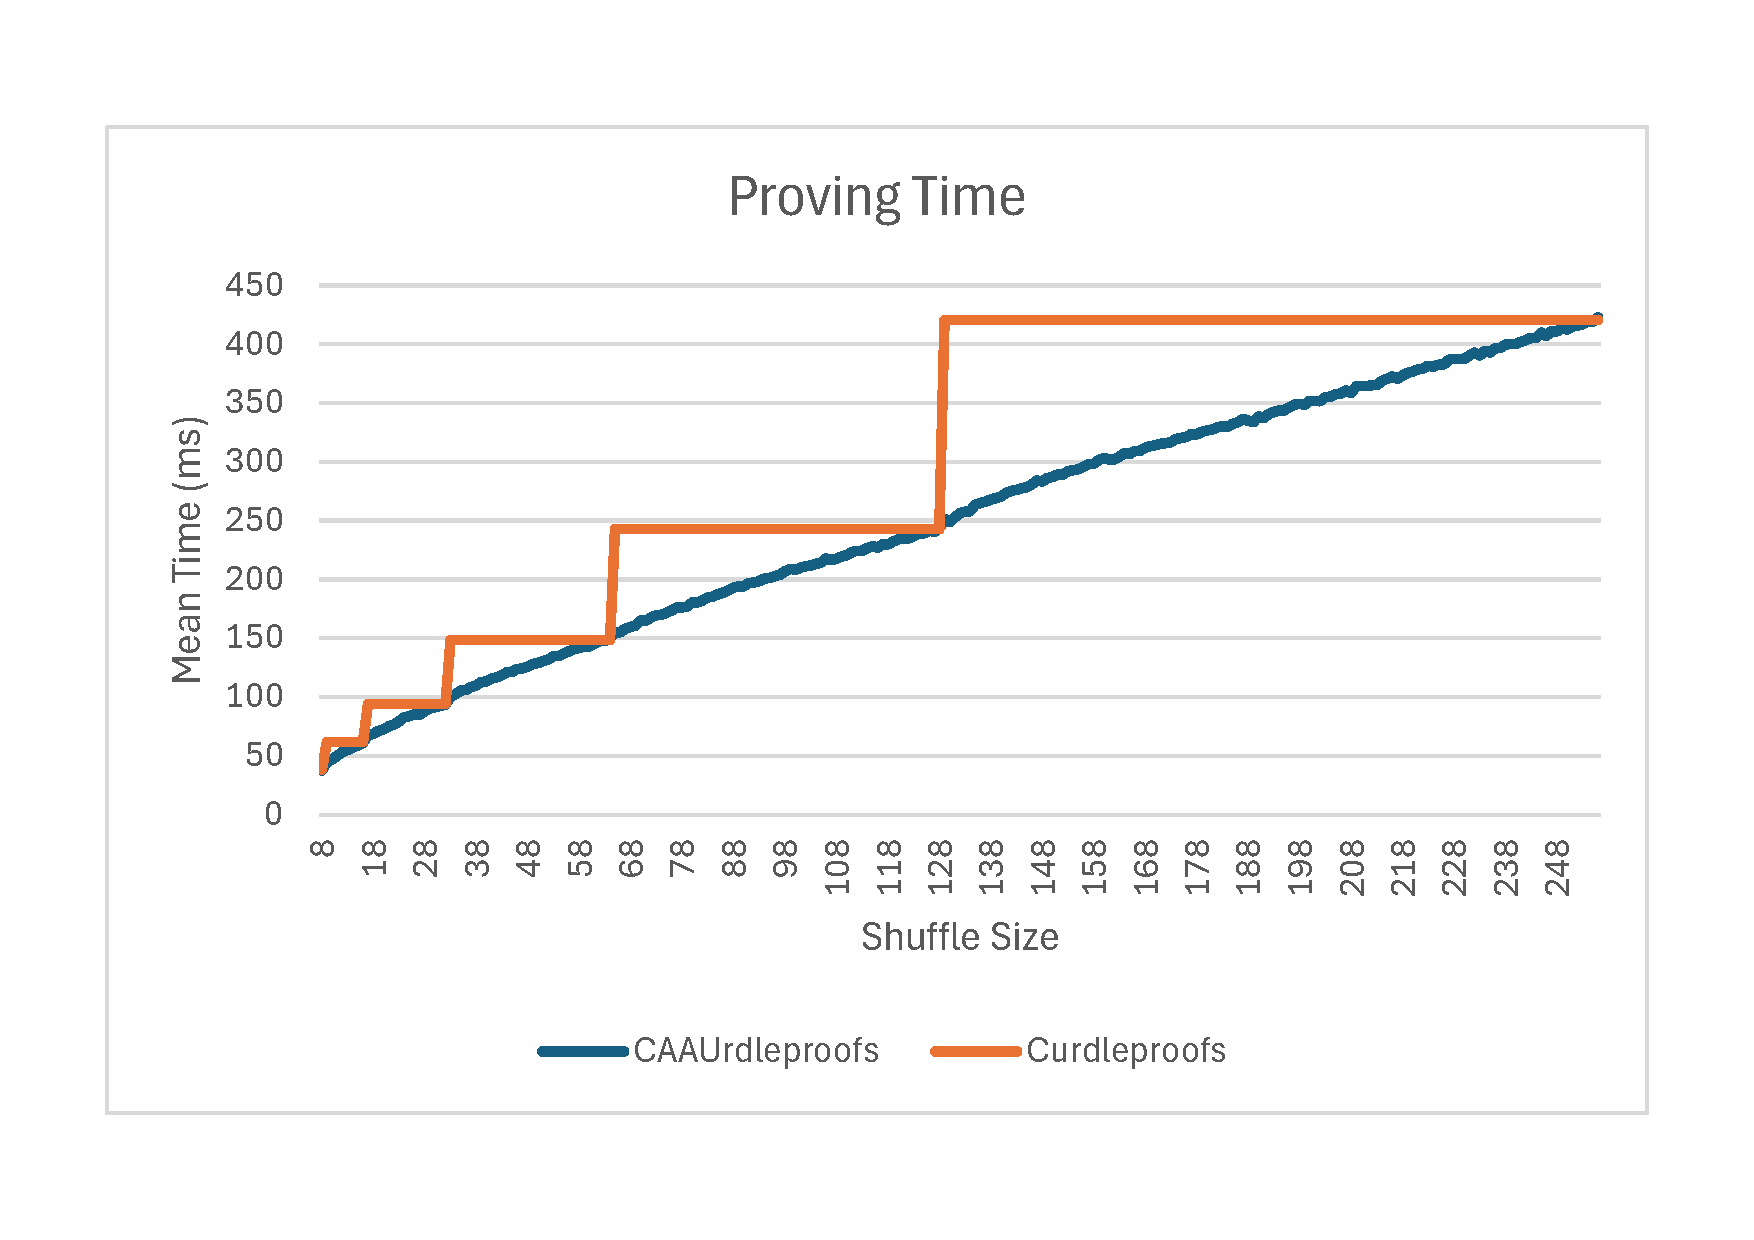
\includegraphics[width=0.45\textwidth]{figures/results/provingtime} }}%
    \qquad
    \subfloat[\centering Verifying Time]{{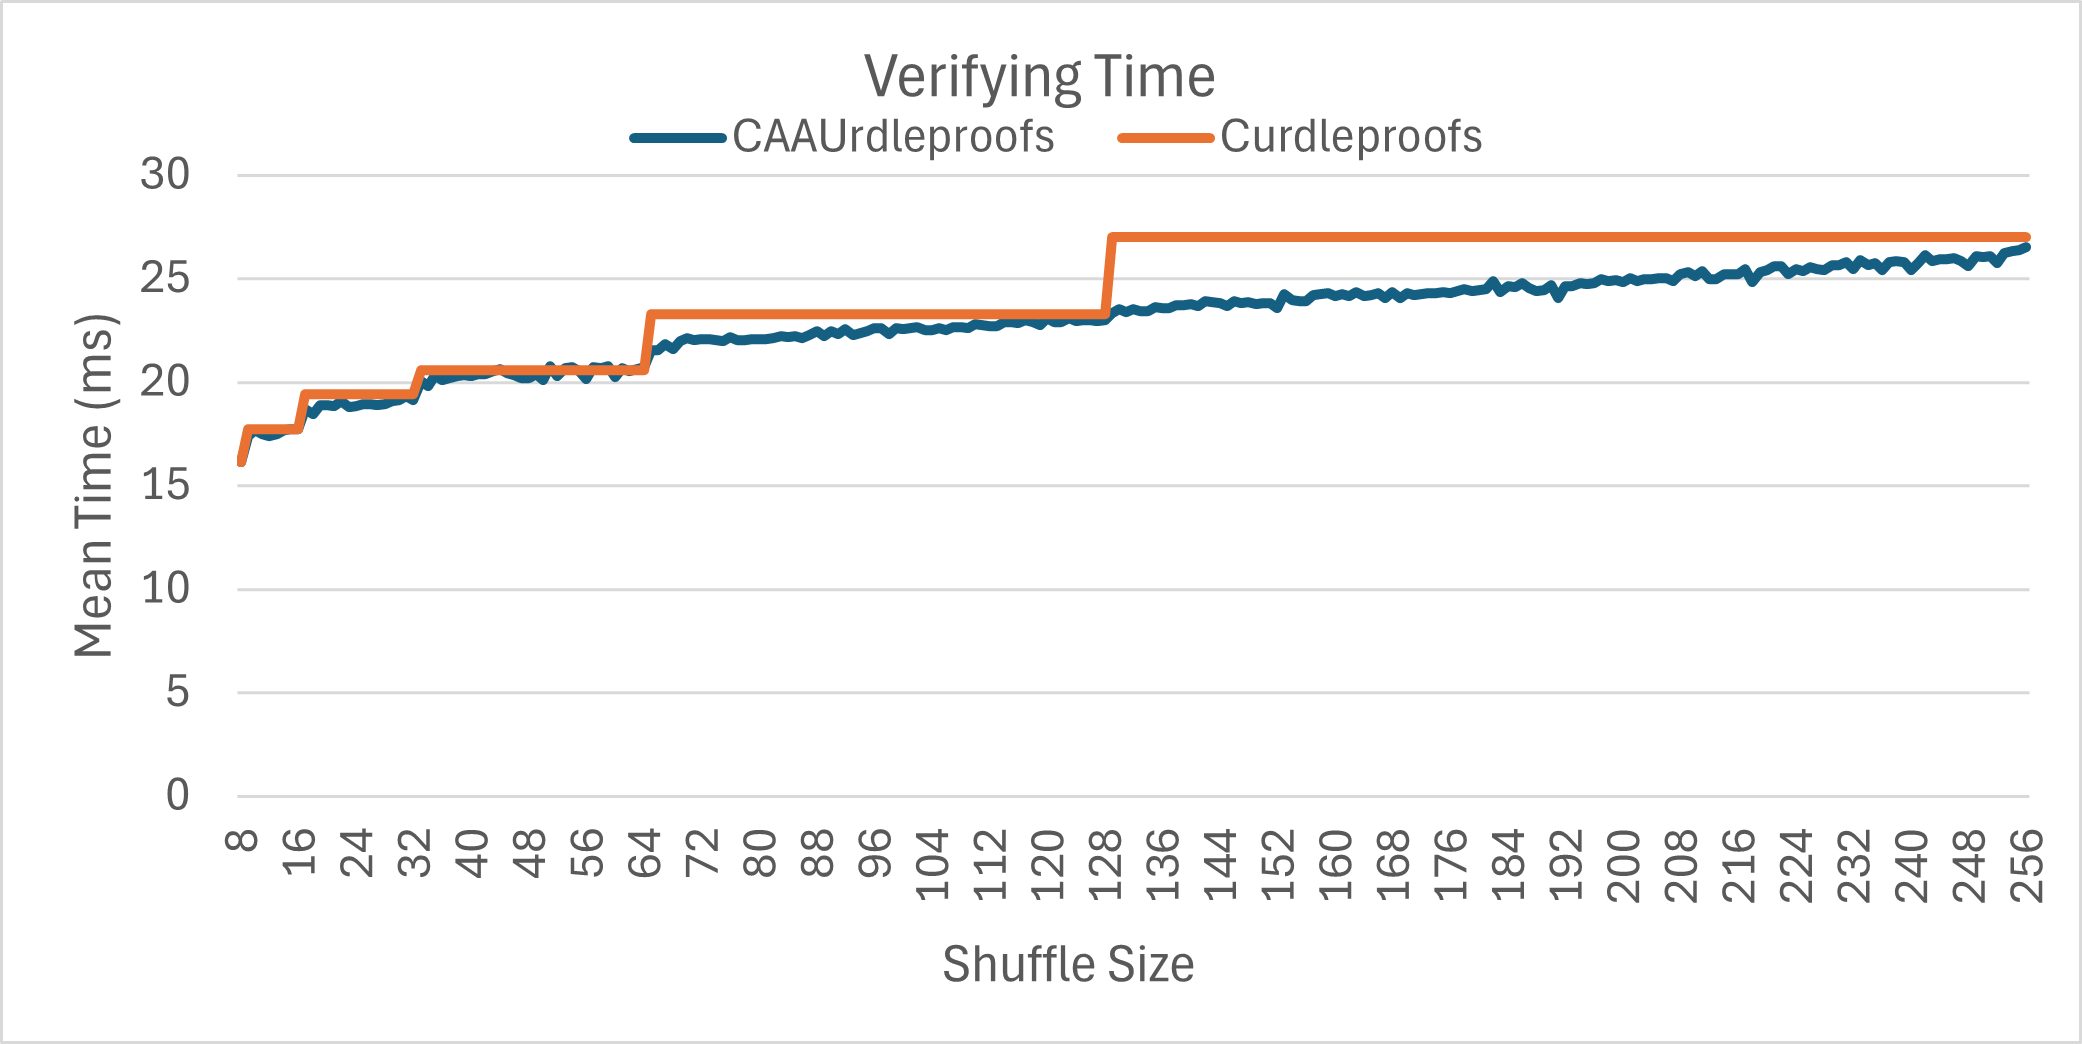
\includegraphics[width=0.45\textwidth]{figures/results/verifyingtime} }}%
    \caption{The timed results compared between CAAUrdleProofs and Curdleproofs}%
    \label{fig:resulttimes}%
\end{figure*}
After running the experiment where Curdleproofs and CAAUrdleproofs were compared across different Shuffle sizes, we obtained the results shown in \autoref{fig:resulttimes}.
As mentioned in \autoref{sec:CAAUrdleproof-experiment}, CAAUdleproofs was run with a shuffle size $k$ of $\{8,9,\dots,256\}$ but Curdleproofs was only run with a shuffle size $k$ of $\{8,16,32,64,128,256\}$.
This is why the results for Curdleproofs instantly goes up to the next size of $k$ because it would have to pad the inputset until it reaches the next size of a power of 2.
From the results, we can see that CAAUrdleproofs and Curdleproofs have similar proving and verifying times when $k$ is a power of 2 but whenever $k$ is not a power of 2 CAAUrdleproofs is faster.


\subsection{Shuffle security}\label{subsec:Shuffle-security}


    

\section{Discussion}\label{sec:discussion}
In this section we will discuss the results of the experiments in \autoref{sec:results} and how they relate to the CAAUrdleproofs protocol.
We will also discuss some of the limitations of the CAAUrdleproofs protocol and how it compares to Curdleproofs.


\subsection{CAAUrdleproofs in comparison to Curdleproofs}\label{subsec:CAAUrdleproofs-vs-Curdleproofs}
As mentioned in~\autoref{subsec:results:provingverifying}, the proving and verifying times between the two protocols are close to identical when $\ell$ is a power of two.
We expect that this is because the added computation is negligible compared to other computations that are present in the original Curdleproofs protocol.

On the prover, there is the addition of the scheme function from Springproofs.
Though, as seen in~\autoref{lst:schemefunc}, the scheme function only makes integer calculations based on $n$, and hence should have a negligible impact compared to the cryptographic group computations.
In addition to that, mentioned in~\autoref{subsec:approach-implementation}, the vector is never practically split in two but instead uses pointers.
Therefore, we avoid having to add new variables to memory in every round.

Also, we mentioned in~\autoref{subsec:approach-implementation} that, every round after the first, runs the same code as Curdleproofs.
Thus, only the first round should be able to introduce some computational overhead.
But, as mentioned before, the overhead should be negligible.

The same kind of explanation can be used to describe the same scenario at powers of two on the verifier side.
Looking at~\autoref{lst:ipa-verifier-optimized}(b), we see that the only difference in computation between CAAUrdleproofs and Curdleproofs stems from the calculation of $\mathbf{s}$.
Comparing line 29 and lines 33--47, it becomes clear that both ways work in $\mathcal{O}(n\log n)$, as they do $m$ computations for each of the $n$ elements.
CAAUrdleproofs does, however, need some more integer variables for splitting as well as an array for keeping track of the vector elements' active positions during recursion.
Nevertheless,~\autoref{fig:resulttimes}(b) shows that this does not have a big, if any, impact on the running time.

However, as mentioned in~\autoref{subsec:results:provingverifying}, when~$\ell$ is just above a power of two, we see some more aggressively increasing verifying times.
We expect this to be a result of~$m$ being set to~$\lceil\log n\rceil$ in line 8 of~\autoref{lst:ipa-verifier-optimized}.
E.g., when~$\ell$ is~$65$, it will have to handle computations from an additional recursive round, in comparison to when~$\ell$ is~$64$.
Additionally, this also explains why the increase in running time flattens when~$\ell$ is increases.

Though the pattern shows that this bump has a decreasing impact on the running time, the higher $\ell$ is, as mentioned in~\autoref{subsec:results:provingverifying}.
In theory, the addition of an extra proof element should introduce a constant amount of work for the verifier.

Therefore, we believe this to be an artifact of memory optimizations done either by hardware or Rust.
This could, for instance, include pre-fetching, in which the memory system can optimize access if it suspects some values in memory are going to be used some time later on\footnote{\href{https://doc.rust-lang.org/core/arch/aarch64/fn._prefetch.html}{https://doc.rust-lang.org/core/arch/aarc.h64/fn.\_prefetch.html} — Accessed: 29/05/2025}.
As $\ell$ increases, the memory system will have more data to predict and optimize memory access.

\subsection{Shuffle Security}\label{subsec:Discution-Shuffle-security}
When looking at the results of the shuffle security experiment in \autoref{fig:shufflesecurity} and \autoref{fig:shufflesecurityviolin}, we can see that when taking into account the standard deviation, the shuffle can still be secure with an~$\ell$ as low as 32 within the 8192 shuffles available.
Even when taking into account the worst case scenario from our experiment, the shuffle will still be secure with an~$\ell$ as low as 42 within the 8192 shuffles available with an $\alpha$ of 8192.

We would however not recommend using an~$\ell$ lower than 80, as here the worst case scenario needs a little under half the available shuffles to be honest in order to be secure.
As seen in~\autoref{fig:shufflesecurity} you would also only need a third of the 8192 shuffles to be honest to get within the one standard deviation.
This would still lead to a reduction of the proving time of 62.69ms, which is 74.25\% of the current Curdleproofs time and a reduction in the verifying time of 0.89ms, which is 96.11\% of the current Curdleproofs time.
It would also reduce the size of the block overhead from 16.656KB to 12.048KB.
Only 72.33\% of the currently calculated size for Curdleproofs.
This would result in saving $\sim 12.11GB$ of space on the blockchain each year.
Some other things to keep in mind when deciding on how many honest shuffles should be necessary to make the shuffle secure is that there are other factors that can affect the security of the blockchain.
One of such factors is some of the know attacks that takes advantage of controlling a large number of validators.
Attacks like the $>-50\%$ stake attack and the $33\%$ finality attack~\cite{EthereumAttackDefense2024} takes advantage of controlling a large number of validators in order to negatively effect the blockchain system.
Because of attacks like these, which rely on controlling a large number of validators, we would recommend that when evaluating how many honest shuffles should be necessary to make the shuffle secure, one should also take into account how many honest validators are necessary to make the blockchain secure.

Another thing to keep in mind is that within the Ethereum system not every validator is owned by a different person.
Some nodes contain multiple validators, and this means that during the shuffling phase, when selecting the 16384 possible proposers, there is a chance that a single node controls multiple of the chosen validators.
This is also possible during the selecting of the shufflers.

From the results we see that the mean starts higher and ends lower for the experiments with a higher $\alpha$.
One of the reasons for the could be the relationship between the number of adversarial tracked cups and the threshold necessary before the shuffle is secure.
Since the threshold is $2/(n-\alpha)$ the higher $\alpha$ is, the higher the threshold for the amount of water allowed in any cup.
Therefore, the higher $\alpha$ is, the less the water needs to be divided be the harder it is to get the initial 1 unit of water divided.
And opposite to this the lower $\alpha$ is, the more evenly the water needs to be divided, and therefore the harder it is to get the every cup below the lower threshold.

    

\section{Conclusion}\label{sec:conclusion}
After looking into the \glspl{zk} \glspl{ssle} protocol Whisk and the Curdleproofs protocol, we found that there was still was room for improvement in the Curdleproofs protocol.
We saw the strict requirement of the shuffle size being a power of two as a limitation, and we wanted to remove this limitation to try to reduce the block overhead related to the protocol.

To do this we looked at Springproofs which allows for \glspl{ipa} to be of any size.
When combining the Curdleproofs protocol with the flexablility of Springporoofs we made the CAAUdleproofs protocol.
The implementation of the CAAUrdleproofs protocol, is a modified version of the Curdleproofs protocol that allows for any shuffle size.

Through our experiments, we found that the CAAUrdleproofs protocol has similar proving and verifying times to the Curdleproofs protocol when the shuffle size is a power of two.
But for any shuffle size that is not a power of two, the CAAUrdleproofs protocol has a performance advantage.

Since CAAUrdleproofs enables the use of any shuffle size, it can be used to reduce the block overhead related to the protocol without having to compromise the security of the protocol.

This is why we think that CAAUrdleproofs is a good alternative to Curdleproofs, as it allows for more flexibility in the choice of shuffle size base things like the size of the block overhead and the proving and verifying times.

    \section{Future work}\label{sec:future-works}
In this section we will focus on where there is still room for improvement in the Whisk protocol.

The main modification from Curdleproofs to CAAUrdleproofs is the added flexibilty in choosing the shuffle size for Whisk.
Hence, a topic for future improvements could be proof structure modifications.
The goal of this is to improve the protocol in all cases.
Also in cases where the shuffle size is a power of two, for which Curdleproofs and CAAUrdleproofs show similar results.
As seen in Appendix~\ref{app:curdleproofs-weighted-inner-product-argument-modification-attempt}, we tried to do this using~\glspl{wipa} instead of~\glspl{ipa}.
Though, we found that there was not enough time to follow through, as it seemed that significant structural changes were needed for this change to be possible.


Besides trying to make the proof faster, and the block overhead smaller, there are also calls for making the protocol more secure.
Specifically, work has already begun trying to make Curdleproofs post-quantum secure~\cite{pqwhisk}.
In this work, they make use of~\gls{csidh}~\cite{10.1007/978-3-030-03332-3_15}.
Isogeny-based cryptography is based on maps between elliptic curves.
Using isogenies, a hard problem comes up, namely the~\gls{gaip}.
\begin{definition}[Group Action Inverse Problem (GAIP)]
    Given a curve $E$, with $End(E)=O$, find an ideal $a\subset O$ such that $E=[a]E_0$
\end{definition}
Using this problem, an almost one to one conversion into using post-quantum cryptography can be done on Whisk, as shown by Sanso~\cite{pqwhisk}.
At the moment, though, there does not exist a~\gls{nizk} proof of shuffle based on isogenies.


With Whisk, a list of upcoming proposers is still chosen and published some time before they are needed for duty.
But because upcoming proposers are published as trackers that only the chosen validator can open and prove ownership of, attacks such as~\gls{dos} attacks are a lot harder to accurately perform.

Though, as found by Heimbach et al.~and confirmed by ourselves, the execution of the~\gls{dos} attack is only half the attack~\cite{heimbach2024deanonymizingethereumvalidatorsp2p,ouroldpaper}.
Even if the blockchain is using Whisk, it is still possible for an adversary to gather and de-anonymize validator IP addresses only by running a node on the network.
A sustainable solution for this therefore needs to be found.
Currently, ideas such as $k$-anonymity, where nodes group together in $k$-size groups and randomize who sends routine messages to the network, have been proposed.

    

\section{Acknowledgements}\label{sec:acknowledgements}
We want to express our sincere gratitude to Daniele Dell'Aglio and Michele Albano for their supervision and guidance throughout this thesis.

We also want to thank the authors of springproofs~\cite{zhang2024springproofs} for supplying their code used which we used for reference when building CAAUdleproofs in this thesis.
Also thanks to the authors of Larsen et al.~\cite{cryptoeprint:2022/560} for being of great help by providing answers to our questions regarding their paper on shuffle security.

We also acknowledge the usage of AI tools such as ChatGPT, GitHub Copilot, and Grammarly.
These have been used for clarification and implementation purposes.

    \clearpage
    %\printglossary[type=\acronymtype]

    \printbibliography

    \appendices % You can use \appendix if you only have a single appendix
    %! Author = Runge
%! Date = 29-12-2023

% Main appendix file
% Insert appendix sections below
%! Author = ander
%! Date = 18-10-2024
\section{Attacks on Ethereum}\label{sec:attacks-on-ethereum}
\subsection{Reorg}\label{subsec:reorg}

\subsection{DoS}\label{subsec:dos}
We've found three different kinds of DoS attacks that either were or are possible to perform on Ethereum.

One of the attacks is called \textit{under-priced opcodes}~\cite{10.1145/3391195,9815256}.
This attack works because Ethereum has a gas mechanism to reduce abuse of computing resources.
Though when a contract has a lot of underpriced opcodes, they will consume many resources.
Execution of contracts requires a lot of resources.

To mitigate this,
Ethereum has raised the gas cost of opcodes
to preserve the number of transactions-per-second~\cite{Opcode-mitigation}~\footnote{
\href{https://github.com/ethereum/EIPs/blob/master/EIPS/eip-150.md}{EIPs/EIPS/eip-150.md at master ethereum/EIPs GitHub}}.

Another attack,
which is closely related to the former, is \textit{empty account in the state trie}~\cite{10.1145/3391195,9815256}.
This attack was possible
because the existence of empty accounts increases the transaction processing time and synchronization.
An empty account is an account with zero balance and no code.
The attack required the proposer to select only the transactions of the adversary,
which could be insured by offering a higher gas price.

The mitigation is a combination of the one
explained for \textit{under-priced opcodes} as well as a mitigation
for clearing empty accounts~\cite{Opcode-mitigation,empty-account-mitigation,empty-account-eip-mitigation}~\footnote{
\href{https://github.com/ethereum/EIPs/blob/master/EIPS/eip-161.md}{EIPs/EIPS/eip-161.md at master ethereum/EIPs GitHub}}.

The last example of a DoS attack is called \textit{Proposer DoS}~\cite{EthereumSSLE2024,EthereumAttackDefense2024}.
The background to making this attack possible is
that the consensus mechanism uses a publicly known function for choosing the upcoming block proposers.
The adversary is therefore able to compute this in slight advance of the blockchain, s.t.\ each proposer is now known.
After this, the adversary can map the proposer's IP addresses and overload their connection.
A successful attack would leave a proposer unable to propose their block in time.

To prevent this kind of attack,
Ethereum plans
to use something they call~\gls{ssle} which ensures
that only the selected validator knows that they have been selected~\cite{EthereumSSLE2024,EthereumResearchSSLE2024}.

Specifically, a proposal has been made to use an election protocol called Whisk, which is a type of~\gls{ssle}~\cite{Whisk2024}\footnote{\href{https://github.com/ethresearch/Shuffle_SSLE/tree/master/rust_code/src}{Shuffle\_SSLE/rust\_code/src at master ethresearch/Shuffle\_SSLE GitHub}}\footnote{\href{https://github.com/ethereum/consensus-specs/pull/2800}{[WIP] Introduce consensus code for Whisk (SSLE) by asn-d6 Pull Request \#2800 ethereum/consensus-specs GitHub}}\footnote{\href{https://github.com/dapplion/lighthouse/tree/whisk}{GitHub - dapplion/lighthouse at whisk}}.
It works by each validator submitting a commitment to a secret shared by all validators.
The commitments are shuffled s.t.\ no-one can map commitments to the validators,
but each validator knows what commitment belongs to them.
This shuffle-phase goes on for a day, 256 epochs, before using the shuffled proposer list the following day.
Commitments are chosen at random, and the selected proposer will detect its commitment to know when to propose a block.

The shuffling phase requires validators to occasionally shuffle a subset of candidate proposers.
Using a subset is a measure to reduce computation for the validators, as 256 epochs correspond to 8912 proposers.
The shuffle requires a validator to construct a~\gls{zkp} to confirm that the shuffle was performed correctly.

\subsection{Balancing Attack}\label{subsec:balancing-attack}
For this type, we found two attacks.

The first attack we call \textit{LMD-specific balancing attack}~\cite{10.1145/3560829.3563560}.
This attack exploits the~\gls{lmd} \textit{proposer
boosting} by sending out two competing blocks
but giving half the validators one block before the other and the opposite for the other half.
This would create a fork in the blockchain.

Although no mitigation is mentioned,
it requires $W_p/b+1$ adversarial slots~\footnote{where $W_p$ is the proposer boost weight (fx 100 validators/slot: $W_p=0.7\cdot100=70$)
    and $b$ is the fraction of adversaries in the committee in each slot}.


Another balancing attack has the adversary
exploiting adversarial network delay
and strategic voting by a vanishing fraction of adversarial validators
to stall the protocol indefinitely~\cite{10.1007/978-3-031-18283-9_28}~\footnote{
\href{https://github.com/tse-group/gasper-gossip-attack}{GitHub - tse-group/gasper-gossip-attack}}.

Though this attack does depend on networking assumptions that are highly contrived in practice; those being the attacker having fine-grained control over latencies of individual validators.

\subsection{Finality Attack (Bouncing Attack)}\label{subsec:finality-attack-(bouncing-attack)}
For the Ethereum, there exists attacks called finality attacks, also known as bouncing attacks, which have the purpose of denying the blockchain to finalize its block, halting its functionality.

The first attack is a \textit{double finality} attack~\cite{EthereumAttackDefense2024, 10646904}.
It is theoretically possible for an attacker that wants to risk 34\% of the total staked ether.
Two forks finalize simultaneously, creating a permanent split of the chain.

A way to see a mitigation of this is that it is practically impossible given the current value of 34\% of the total staked ether.
Also, voting on two different chains, called double voting, is a slashable offense in the Ethereum chain, so the adversary would get their staked ETH slashed.


Another finality attack is called \textit{33\% finality attack}~\cite{EthereumAttackDefense2024}.
Here, all adversarial ($\geq33\%$) validators can simply go inactive, meaning that a block cannot get $2/3$ attestations which is required to achieve finality.
Therefore, the blockchain would not be able to go further, as it would not be able to achieve finality.

The mitigation for this is called \textit{the inactivity leak}.
The Ethereum chain penalizes the validators who resist voting or are inactive.
Their ETH gets burned until the majority vote has a 2/3 majority.
This makes the attack impractical for the attacker, as it is costly to have $\geq33\%$ of the total staked ETH and their ETH gets burned as well.

\subsection{Avalanche Attack}\label{subsec:avalanche-attack}

\subsection{Bribery}\label{subsec:bribery}

\subsection{Staircase Attack}\label{subsec:staircase-attack}

\end{document}
